\section{Многолучевые алгоритмы оценки угла прихода сигнала в системе 5G NR}
\subsection[Иерархический поиск с минимизацией СКО]{Иерархический поиск с минимизацией СКО -- \hSearchMMSE}
\label{sec:hSearchMMSE:multipath}

Однолучевая версия алгоритма hSearchMMSE, описаная в разделе
\ref{sec:hSearchMMSE:singlepath},
может быть расширина на многолучевую.  Однако, этот алгоритм есть аппроксимация
метода Фурье (непрерывного сканирования лучом), hSearchMMSE имеет характерные
недостатки.
Во-первых, разрешение ограничено шириной луча, но в контексте нашей
системы это не настолько критично. Второй недостаток более серьезный, он связан
с эффектов утечки мощности через боковые лепестки ДН.  Это означает, что мы
можем ошибочно распознать основной путь распространения, обнаруженный боковым
лепестком, как запасной путь.  Чтобы избежать подобной ошибки, необходимо
установить порог мощности для обнаружения запасного пути. Этот порог должен
учитывать утечку мощности через боковые лепестки и шумовое воздействие.

\begin{equation}
    \label{eq:4.57}
    Th_1^{mn} = A_n
    \frac
    {\sin^2(0.5 N (\eta_u - \hat \psi_1))}
    {\sin^2(0.5 (\eta_u - \hat \psi_1))} + 9 \sigma^2,
\end{equation}
\begin{equation}
    \label{eq:4.58}
    Th_2^{mn} = G A_n \frac{\sin^2(0.5 N (\eta_u - \hat \psi_1))}
    {\sin^2(0.5 (\eta_u - \hat \psi_1))} + 9 \sigma^2,
\end{equation}
где $n$ -- индекс луча базовой станции, $n$ -- индекс луча пользователя, $A_n$
-- <<мощность>> основного луча, включающая в себя ДН базовой станции, $G$ --
ослабление мощности элемента антенной решетки при приеме тыльной стороной
решетки ($-23$ дБ), $\eta_u$ -- направление луча пользователя в обобщенных
координатах, $\hat \psi_1$ -- оцененный угол прихода основного луча, $\sigma^2$
-- мощность шума, множитель $9$ добавлен исходя из правила $3\sigma$.
Идея второго слагаемого в выражениях \eqref{eq:4.57},\eqref{eq:4.48} в том,
чтобы уменьшить вероятность ложной тревоги из-за шума.
Порог $Th_1$ используется
для следящей решетки, той на которой был определен основой луч, а порог $Th_2$
для запасной решетки.  Величина $A_n$ может быть оценена, используя уравнение
\begin{equation}
      \label{eq:4.59}
    A_n = \frac{1}{M+1} \sum\limits_{m=-M/2}^{M/2} \hat p_{mn}
    \frac{\sin^2(0.5(\hat \psi_1 - \chi_m))}{0.5 N_{rx}(\hat \psi_1 - \chi_m)},
\end{equation}
где $\chi_m$ -- обобщенный угол, найденный на этапе сканирования
(см. раздел \eqref{sec:hSearchMMSE:singlepath}), $\hat p_{mn}$ --
измеренная мощность на $m$-ом луче UE во время этапа дополнительных измерений и
$n$-ом луче BS.
Стоит отметить, что $A_n$ для каждого луча оченивается независимо.

Пошагово алгоритм выглядит следующим образом.
\begin{enumerate}[label=\textbf{Шаг \arabic*:}]
    \item BS производит сканирование лучом. UE последовательно использует
          каждый луч из кодовой книги \eqref{eq:4.16}
          для измерения мощности на каждом луче BS.  Эта процедура
          выполняется для AIP1 и AIP2. Мощность измерения на этом этапе
          сохраняется в матрицах $\vec P_1$ и $\vec P_2$ соответственно.
          Каждый элемент матрицы соответствует
          определенным парам лучей UE и BS.
    \item Выбирается лучшая пара лучей UE-BS. Обозначим обобщенный угол
          лучшего луча как $\eta_{v1}$ и индекс лучшего луча BS как
          $q_1$.
    \item Тестируются гипотезы $H_1$, $H_2$, $H_3$ (см. рис. \ref{fig:4.14}) с
          помощью \eqref{eq:4.34}. Мощность на соседний лучах пользователя
          ($u=v-1$, $u=v+1$) измеряется на одинаковых лучах BS с индексом
          $q_1$. Выбирается гипотеза с наибольшей метрикой \eqref{eq:4.34}.
    \item БС периодически сканирует своими лучами.
          UE последовательно использует каждый луч кодовой книги (4.19) для
          измерить мощность для каждого луча БС. Если выбрана гипотеза $H_2$,
          (4.20) используется для формирования кодовой книги.
          В противном случае используется (4.33).
          Знак <<->> соответствует $H_1$. Знак <<+>> соответствует H3
    \item Мы выполняем алгоритм поиска, представленный в листинге \ref{lst:4.1}, используя
          условие MMSE \eqref{eq:4.31}).
          Мы используем мощность измеряется для лучшего луча на
          шаге 2 и лучей на шаге 4. Предполагается, что луч БС одинаков.
          как в лучшей
          паре на шаге 2 (т.е. имеет индекс q1). Пусть $\hat \psi_1$ --
          предполагаемая пространственная частота первого путь распространения
    \item Выполняется оценка <<мощности>> используя \eqref{eq:4.59} для
          каждого луча БС.
    \item Выбираем максимальный элемент матриц $P_1$ или $P_2$ (другая пара лучей
          UE-BS), который превышают пороги \eqref{eq:4.57} или \eqref{eq:4.58}.
          Пусть это будут индексы
          ($v_2$ и $q_2$).
          Обратите внимание, что если AIP2 обнаружил основной путь, порог
          $Th_1$ применяется для матрицы $P_2$ (т.е. $P_{2un} > Th_{1un}$) и наоборот.
          Также мы должны исключить элементы, соответствующие балке, которая была
          выбрана на шаге 2 ($v_1$) для соответствующий АИП. Если выбранный луч
          $v_2$
          является соседом $v_1$, влияние основного пути на угол атаки оценка
          чрезмерно высока (утечка боковых лепестков). Таким образом, в этом
          случае мы предлагаем изменить AIP и выберите другую лучшую пару лучей.
          Пусть это также будет ($v_2$ и $q_2$).
    \item Мы проверяем гипотезы $H_1$, $H_2$ и $H_3$ для пары лучей, выбранной
          на шаге 7. Гипотеза $H_1$ не проверено, если мы выбрали первый луч UE ($v_2
              = 1$) или луч с индексом ($v_2 = v_1+1$). Гипотеза $H_3$ не тестируется,
          если мы выбрали последний луч UE ($v_2 = 8$) или луч с индексом
          $(v_2 = v_1-1)$.
    \item БС периодически сканирует своими лучами. UE последовательно использует каждый луч кодовой книги (4.19) для
          измерить мощность для каждого луча БС. Если выбрана гипотеза $H2$,
          \eqref{eq:4.20} используется для формирования кодовой книги.
          В противном случае используется \eqref{eq:4.33}.
          Знак <<->> соответствует $H_1$. Знак <<+>> соответствует $H_3$.
    \item Мы выполняем алгоритм поиска, представленный в листинге \ref{lst:4.1},
          используя условие MMSE \eqref{eq:4.31}. В уравнение подставляем мощность,
          измеренную для луча, выбранного на шаге 7, и лучей на шаге 9. Луч БС
          предполагается таким же, как и в выбранной паре на шаге 7 (т.е. имеет индекс
          $q_2$). Пусть $\hat \psi_2$ оценивается пространственно частота первого пути
          распространения.
    \item Мы рассчитываем АОА на основе оценок пространственных частот $\hat \psi_1$ и
          $\hat \psi_2$. Если выбрана пара лучей UE-BS связанная с AIP1, $\hat \phi_{AOA}=\hat \phi$
          используя \eqref{eq:4.21}.
          Если она связана с AIP2, $\hat \phi_{AOA} = \hat\phi + \pi$. Результат
          получается в радианах.
\end{enumerate}

Временн\'{а}я диаграмма описанноого алгоритма представлена на рис. \ref{fig:4.25}.
Параметры алгоритма представлены в таб. \ref{tab:4.6}.

\begin{figure}[h!]
    \centering
    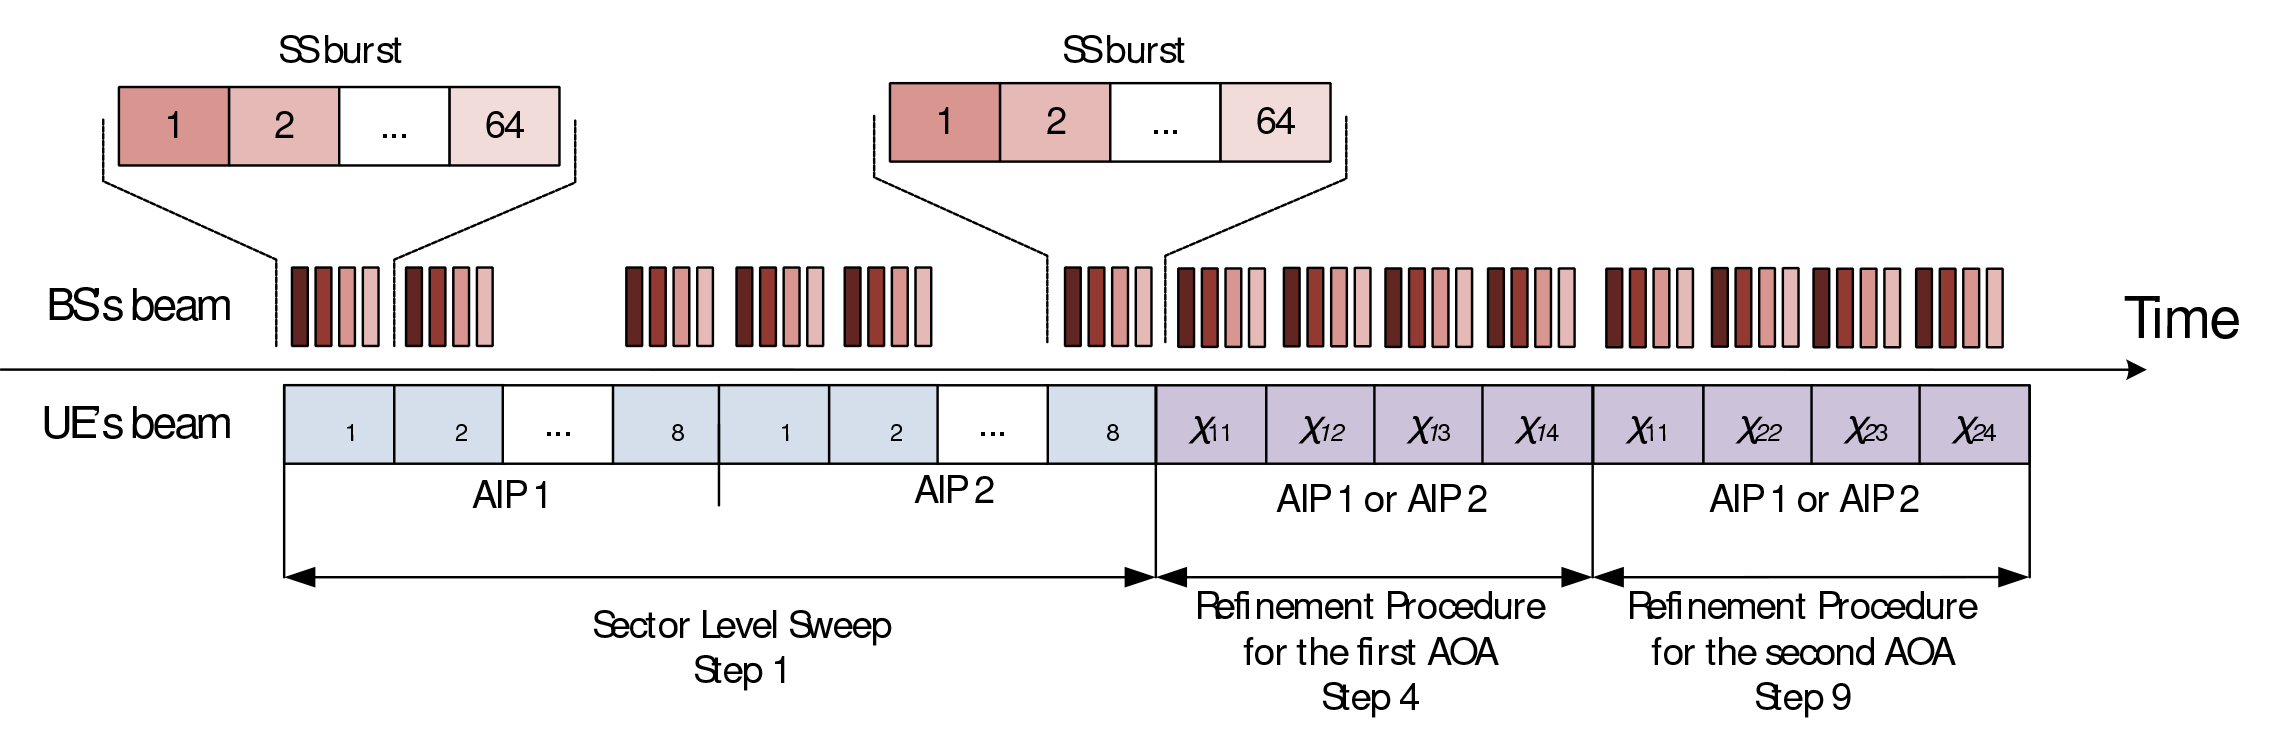
\includegraphics[width=\linewidth]{figs/fig4.25}
    \caption{}
    \label{fig:4.25}
\end{figure}

\begin{table}[h!]
    \centering
    \caption{Параметры многолучевого алгоритма hSearchMMSE}
    \label{tab:4.6}
    \begin{tabular}{lcc}
        \toprule
        \midrule
        Структура RS                         & SS burst  & CSI-RS       \\
        N / M / AIPs                         & 8 / 4 / 2 & 8 / 2 / 2 /2 \\
        Число просканированных лучей (UE/BS) & 24 / 64   & 20 / 8       \\
        Суммарное число RS                   & 1536      & 160          \\
        Необходимое время (слот 0.125 мс)    & 464 мс    & 40 мс        \\
        \hline
    \end{tabular}
\end{table}



\subsection[Модифицированный моноимпульс]{Модифицированный монопульс -- \AuxBeam}
\label{sec:AuxBeam:multipath}


Алгоритм вспомогательного луча (см. \ref{sec:AuxBeam:singlepath})
может быть расширен в многолучевом
случае аналогично тому, как hSearchMMSE (см. \ref{sec:hSearchMMSE:multipath}).
На этот алгоритм также влияют сильно боковые лепестки ДН, но эта проблема
может быть решена порогом, описанным выше. Мы предоставляем здесь
детальное описание алгоритма.

\begin{enumerate}[label=\textbf{Шаг \arabic*:}]
    \item БС прозванивает все свои лучи, UE последовательно использует
          каждый вектор кодовой книги \eqref{eq:4.16} и \eqref{eq:4.17} для
          измерения мощности на каждом луче БС. Измеренная мощность сохраняется
          в матрицах $\vec P_1, \vec P_2$ соответственно. Каждый элемент матрицы соответствует
          определенной паре лучей UE-BS.
    \item Выбирается лучшая пара лучей UE-BS на основе измеренной мощности.
          Обозначим лучший луч UE индексом $v_1$, а лучший луч BS -- $q_1$.
          Для одинаковых лучей BS выбирается сильнейшний луч, соседний лучшему.
          Обозначим этот луч $w_1$. Вычисляется метрика \eqref{eq:4.39}, где $u=\min(v_1,w_1)$.
          Пример выбранных лучей пользователя показан на рис. \ref{fig:4.17} цветными линиями.
    \item Если условие на доверительный интервал $\zeta_{low} < \hat \zeta_1 < \zeta_{up}$
          выполняется (см. \eqref{eq:4.39}), производится оценка обобщенного угла прихода
          $\psi_1$ с помощью \eqref{eq:4.41} и шаг 4 пропускается.
    \item Обозначим $\eta_{v_1}$ обобщенный угол лучшего луча пользователя.
          На этом шаге производятся дополнительные измерения в направлениях
          $\eta_{v_1 - 0.5} = \eta_{v_1} - \delta$ и
          $\eta_{v_1 + 0.5} = \eta_{v_1} + \delta$. Дополнительные лучи
          показаны на рис. \ref{fig:4.17} пунктирными линиями. Далее вычисляется
          метрика \eqref{eq:4.39} для этих лучей ($u=v_1 - 0.5$) и оценивается
          обобщенный угол прихода $\psi_1$, используя \eqref{eq:4.41}
    \item Оценивается <<мощность>> основного пути распространения \eqref{eq:4.59} для каждого луча BS.
    \item Выбираются максимальные значения из матриц $\vec P_1, \vec P_2$,
          превышающие пороги \eqref{eq:4.57} или \eqref{eq:4.58}. Пусть выбранные значения соответствуют
          индексам $v_2\neq v_1$ и $q_2 \neq q_1$.  Отметим, что если $\psi_1$ был
          обнаружен на второй АР, то порог $Th_1$ применяется для матрицы $P_2$ и наоборот.
    \item Для одинаковых лучей BS с индексом $q_2$ выбирается сильнейшний сосед луча UE
          с индексои $v_2$. Обозначим индекс этого соседа $w_2$. Если $w_2 = v_1$ или $w_2=w_1$,
          невозможно корректно завершить алгоритм поиска запасного луча. Поэтому предлагается
          выбрать другую АР и найти два самых сильных соседних луча $v_2$ и $w_2$.
    \item Используя измеренную мощность с шагов 6 и 7, вычисляется метрика \eqref{eq:4.39},
          где $u=\min(v_2,w_2)$.
    \item Если выполняется условие на доверительный интервал $\zeta_{low} < \hat \zeta_2 < \zeta_up$,
          оценивается обобщенный угол прихода $\hat \psi_2$ используя \eqref{eq:4.41} и шаг 10 пропускается.
    \item Пусть $\eta_{v_2}$ -- обобщенный угол сильнейшего луча пользователя, выбранного на шаге 6 или 7.
          Выполняются дополнительные измерения в направлениях
          $\eta_{v_2 - 0.5} = \eta_{v_2} - \delta$,
          $\eta_{v_2 + 0.5} = \eta_{v_2} + \delta$ и вычисляется метрика \eqref{eq:4.39}
          для этих направлений ($u=v_2 - 0.5$) и оценивается $\hat \psi_2$.
    \item Рассчитывается АОА на основе оценок пространственных частот $\hat \psi_1$ и
          $\hat \psi_2$. Если выбрано UE- Пара лучей БС связана с АИП1, $\hat \phi_{AOA}=\hat \phi$
          определенной в \eqref{eq:4.21}.
          Если это связано с AIP2, $\hat \phi_{AOA} = \hat\phi + \pi$. Результат
          получается в радианах.
\end{enumerate}

\begin{table}
    \centering
    \caption{Параметры алгоритма AuxBeam}
    \begin{tabular}{lcc}
        \toprule
        \midrule
        Структура RS                         & SS burst             & CSI-RS            \\
        N / M / AIPs                         & 8 / 0,2  или 4/2     & 8 / 0,2 или 4/2   \\
        Число просканированных лучей (UE/BS) & 16,18 или 20/64      & 16 / 18  или 20/8 \\
        Суммарное число RS                   & 1024, 1152 или 1280  & 128, 144 или 160  \\
        Необходимое время (слот 0.125 мс)    & 304, 344, или 384 мс & 32, 36 или 40 мс  \\
        \hline
    \end{tabular}
\end{table}
\begin{figure}[h!]
    \centering
    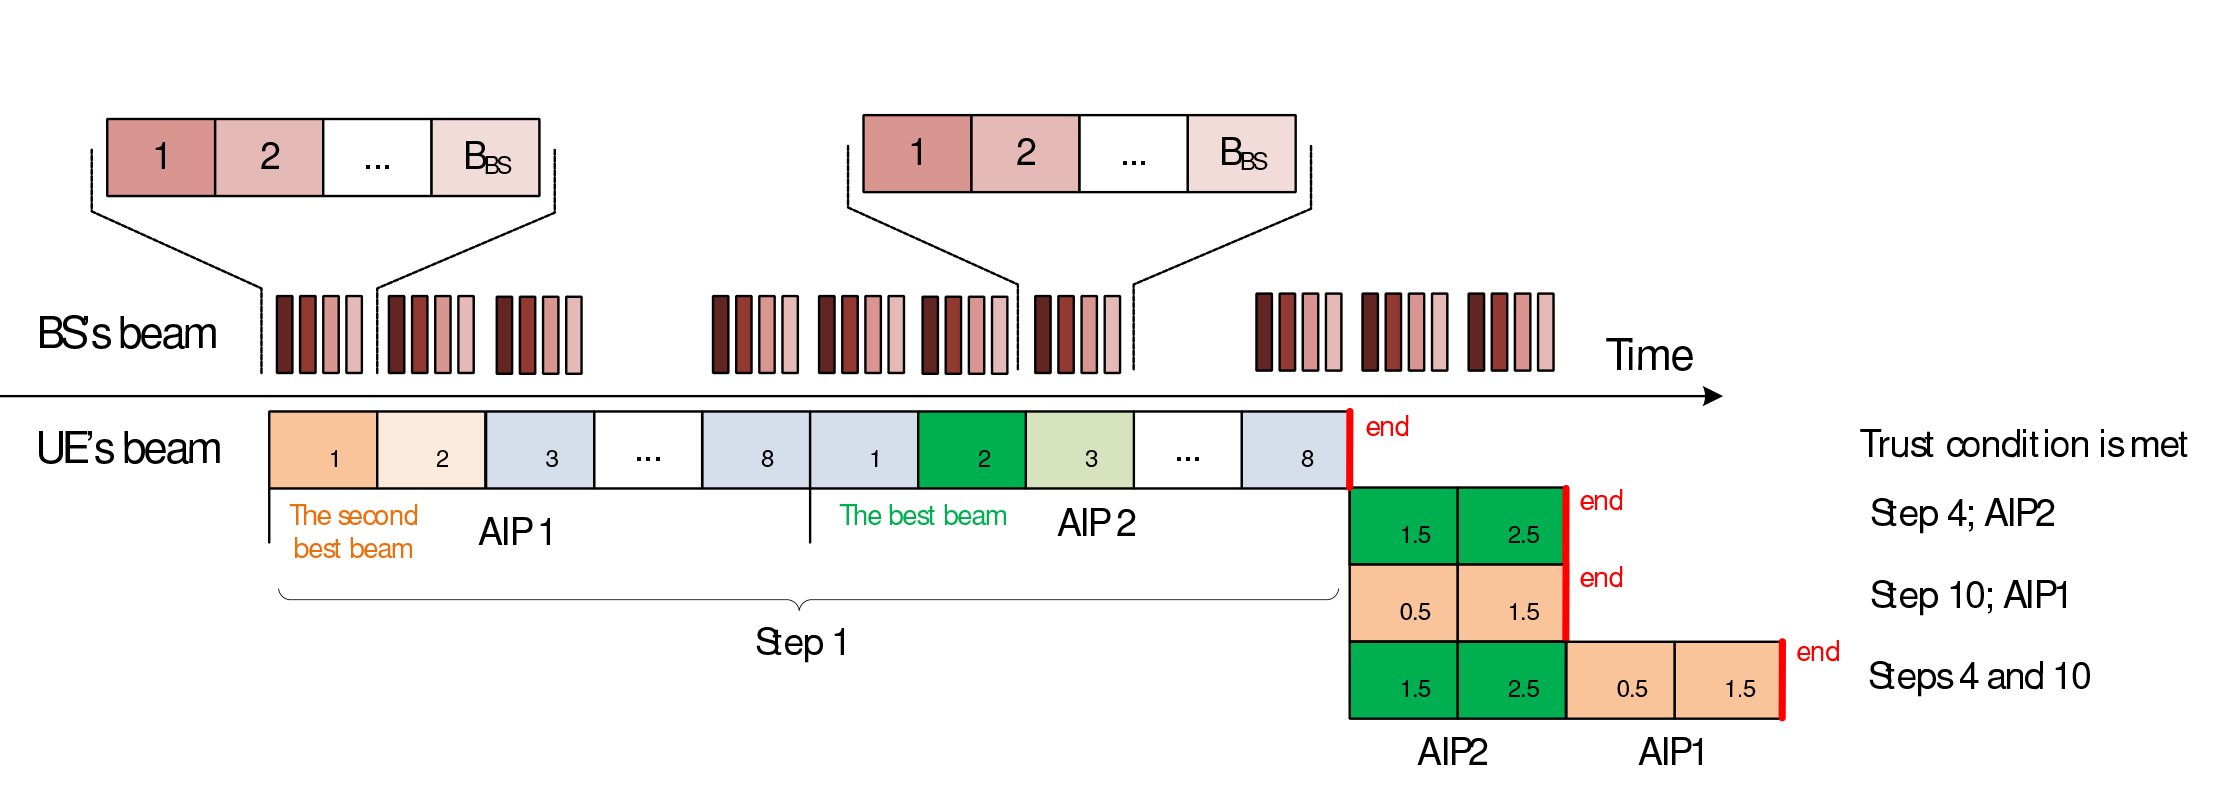
\includegraphics[width=\linewidth]{figs/fig4.26}
    \caption{}
    \label{fig:4.26}
\end{figure}

\subsection[Модифицированный алгоритм бисекций]{Модифицированный алгоритм бисекций -- \ACS}
\label{sec:Compressive:multipath}
В случае многолучевого распространения сигнала вектор $\vec a$  (см. \eqref{eq:4.45}) содержит
несколько ненулевых элементов. Предположим, что ненулевых элементов всего два, что соответствует 
двум возможным путям распространения.
В соответствии с \cite{Alkhateeb2014}, на 
каждой итерации поиска следует разделить вектор $\vec a$ на четыре части и
выбрать две лучших из них.  Физическая интерпретация этой процедуры поиска
представлена на рис. \ref{fig:4.27}, где каждый сектор соответствует определенной
ДН в соответствии с правилом генерации кодовой книги. Таким
образом, на каждом уровне алгоритма мы измеряем четыре разных луча и выбираем
два лучших, чтобы разделить каждый из них на две половины.
\begin{figure}[h!]
    \centering
    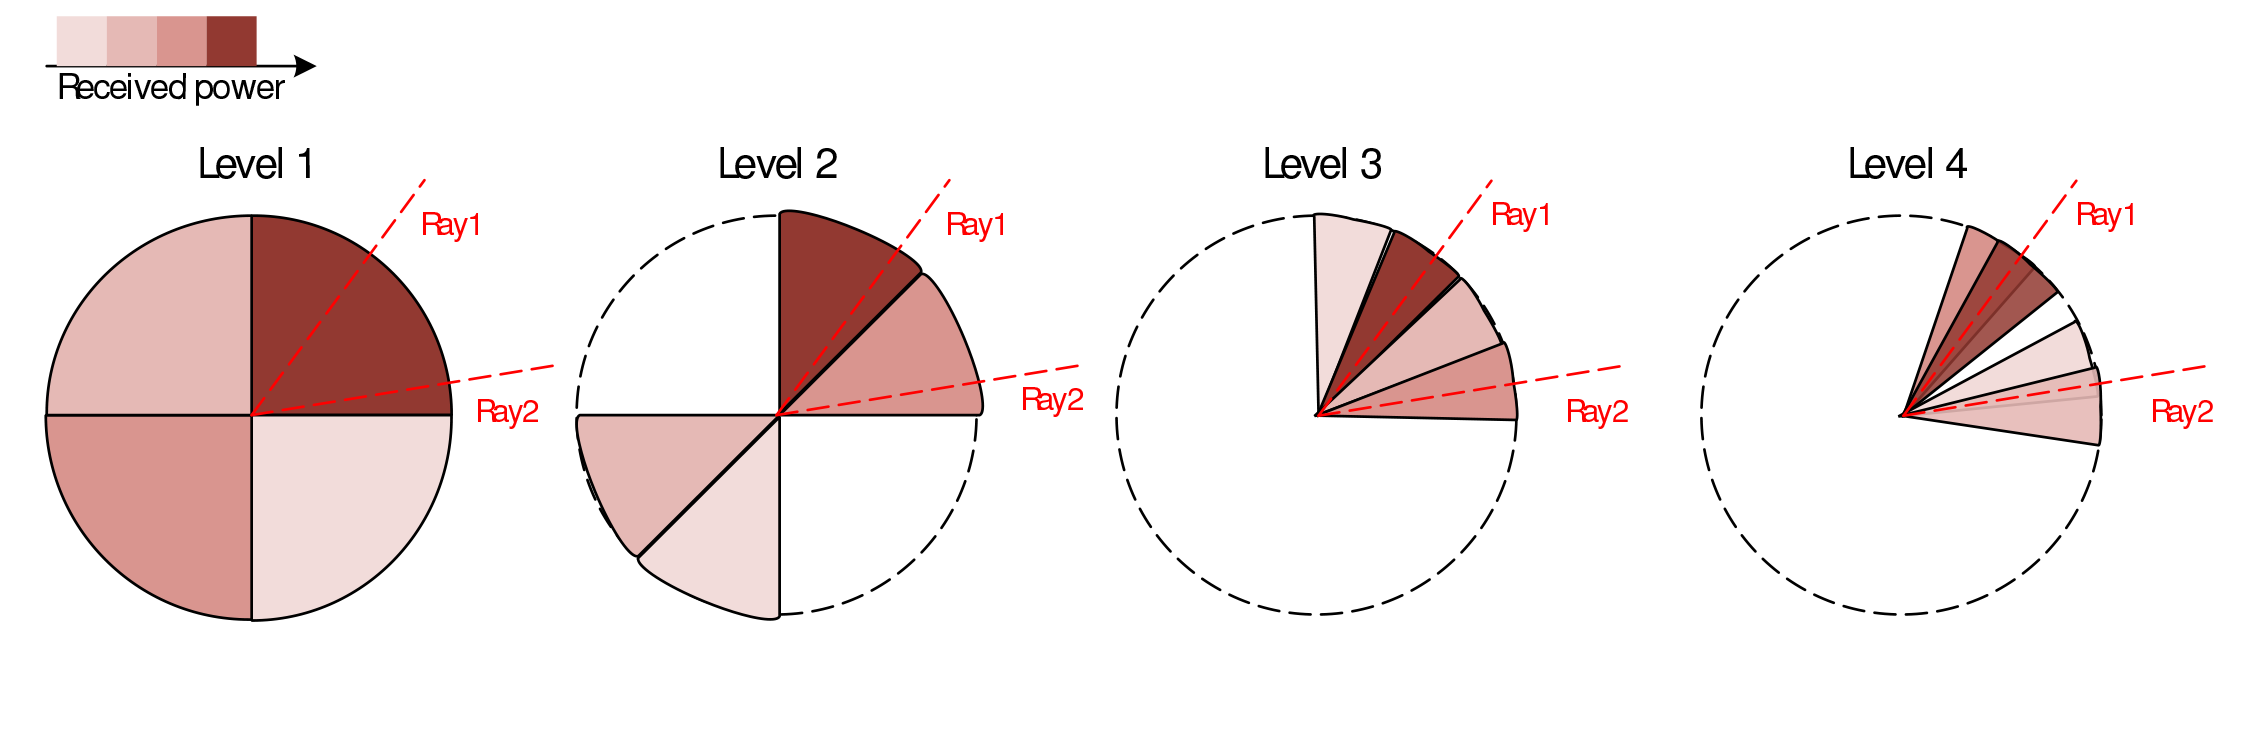
\includegraphics[width=\linewidth]{figs/fig4.27}
    \caption{}
    \label{fig:4.27}
\end{figure}
Однако, после 3-ей итерации ширина ДН перестает меняться из-за недостаточного количества 
элементов в АР пользователя. Получается, что 
во время работы алгоритма <<запасным>> лучом всегда будет выбираться
луч лежащий в одном кластере с основным лучом. 

Для решения этой проблемы предлагается следующая модификация.
Далее предполагается, что обобщенный угол $-\pi < \eta < \pi$ соответвует первой АР, 
а обобщенный угол $\pi < \eta < 3\pi$ -- второй АР.
\begin{enumerate}[label=\textbf{Шаг \arabic*:}]
    \item Уровень 1. БС независимо переключает свои лучи. Введем $\eta_1 = -\pi/2$, 
    $\eta_2 = + \pi/2$, $\eta_3 = 3\pi/2$ и $\eta_4 = 5\pi/2$. Пользователь измеряет принятую мощность 
    на каждом луче БС и каждом луче из следующей кодовой книги  
          \begin{equation}
              \vec W =
              \begin{pmatrix}
                  \mqty{
                  1 & \exp{i\eta_1}      \\
                  1 & \exp{i\eta_2}      \\
                  1 & \exp{i\eta_3}      \\
                  1 & \exp{i\eta_4}      \\
                  }
                    & \mqty{\zmat{4}{6}}
              \end{pmatrix}^T
          \end{equation}
    Пусть $\eta_{v_1}$ и $\eta_{v_2}$ -- обобщенные углы, в направлении которых 
    была принята наибольшая мощность на этом шаге.
    \item
          \begin{equation}
              \vec W =
              \begin{pmatrix}
                  \mqty{
                  1 & \exp{i\eta_1}      & \exp{i2\eta_1} & \exp{i3\eta_1} \\
                  1 & \exp{i\eta_2}      & \exp{i2\eta_2} & \exp{i3\eta_2} \\
                  1 & \exp{i\eta_3}      & \exp{i2\eta_3} & \exp{i3\eta_3} \\
                  1 & \exp{i\eta_4}      & \exp{i2\eta_4} & \exp{i3\eta_4} \\
                  }
                    & \mqty{\zmat{4}{4}}
              \end{pmatrix}^T
          \end{equation}
    \item Уровень 2. БС независимо переключает свои лучи. Введем $\eta_1 = \eta_{v_1}-\pi/4$, 
    $\eta_2 = \eta_{v_1} + \pi/4$, $\eta_3 = \eta_{v_2} - \pi/4$ и $\eta_4 = \eta_{v_2} + \pi/4$. 
    Пользователь измеряет принятую мощность на каждом луче БС и каждом луче из
    следующей кодовой книги  
          \begin{equation}
              \vec W =
              \begin{pmatrix}
                  \mqty{
                  1 & \exp{i\eta_1} & \exp{i2\eta_1} & \dots & \exp{i7\eta_1} \\
                  1 & \exp{i\eta_2} & \exp{i2\eta_2} & \dots & \exp{i7\eta_2} \\
                  1 & \exp{i\eta_3} & \exp{i2\eta_3} & \dots & \exp{i7\eta_3} \\
                  1 & \exp{i\eta_4} & \exp{i2\eta_4} & \dots & \exp{i7\eta_4} \\
                  }
              \end{pmatrix}^T
          \end{equation}
    Обновляются значения $\eta_{v_1}, \eta_{v_2}$.
    \item БС независимо переключает свои лучи. Введем $\eta_1 = \eta_{v_1}-\pi/2^l$, 
    $\eta_2 = \eta_{v_1} + \pi/2^l$, где $l$ -- индекс текущего уровня. После шагом 3 и 4, $l=4$. 
    Пользователь измеряет принятую мощность на каждом луче БС и каждом луче из
    следующей кодовой книги  
          \begin{equation}
              \vec W =
              \begin{pmatrix}
                  \mqty{
                  1 & \exp{i\eta_1} & \exp{i2\eta_1} & \dots & \exp{i7\eta_1} \\
                  1 & \exp{i\eta_2} & \exp{i2\eta_2} & \dots & \exp{i7\eta_2} \\
                  }
              \end{pmatrix}^T
          \end{equation}
    Обновляется $\eta_{v_1}$ и повторяется шаг 4 до тех пор, пока не будет 
    достигнута необходимая точность. Получаем $\hat \psi_1 = (\eta_{v_1} + \pi)\mod(2\pi) - \pi$, где $(x \mod  y)$ -- остаток от деления $x$ на $y$.
    \item БС независимо переключает свои лучи. Введем $\eta_3 = \eta_{v_2}-\pi/2^l$, 
    $\eta_4 = \eta_{v_2} + \pi/2^l$, где $l$ -- индекс текущего уровня. На текущем шаге $l=4$. 
    Пользователь измеряет принятую мощность на каждом луче БС и каждом луче из
    следующей кодовой книги  
          \begin{equation}
              \vec W =
              \begin{pmatrix}
                  \mqty{
                  1 & \exp{i\eta_3} & \exp{i2\eta_3} & \dots & \exp{i7\eta_3} \\
                  1 & \exp{i\eta_4} & \exp{i2\eta_4} & \dots & \exp{i7\eta_4} \\
                  }
              \end{pmatrix}^T
          \end{equation}
    Обновляется $\eta_{v_2}$ и повторяется шаг 5 до тех пор, пока не будет 
    достигнута необходимая точность. Получаем $\hat \psi_2 = (\eta_{v_2} + \pi)\mod(2\pi) - \pi$, где $(x \mod  y)$ -- остаток от деления $x$ на $y$.
    \item Из оцененных $\hat \psi_1$ и $\hat \psi_2$, вычисляются углы прихода. Если $-\pi < \eta_v < \pi$, 
    $\hat \phi_{AOA} = \hat \phi$. Если $\pi < \eta_v < 3\pi$, $\phi_{AOA} = \hat \phi + \pi$.
\end{enumerate}
\begin{table}[h!]
    \centering
    \caption{Параметры алгоритма ACS}
    \begin{tabular}{lcc}
        \toprule
        \midrule
        Структура RS                         & SS burst & CSI-RS \\
        N / M / AIPs                         & 8        & 8      \\
        Число просканированных лучей (UE/BS) & 32/64    & 32/8   \\
        Суммарное число RS                   & 2048     & 256    \\
        Необходимое время (слот 0.125 мс)    & 624 мс   & 64 мс  \\
        \hline
    \end{tabular}
\end{table}
